% Unofficial University of Lethbridge Poster template.
% A fork of unofficial University of Alberta Poster template: 
% which is a fork of Yale template: https://www.overleaf.com/latex/templates/yale-poster-template/rjpgqfgvsjcv
% which is a fork of the UMich template https://www.overleaf.com/latex/templates/university-of-michigan-umich-poster-template/xpnqzzxwbjzc
% which is fork of the MSU template https://www.overleaf.com/latex/templates/an-unofficial-poster-template-for-michigan-state-university/wnymbgpxnnwd
% which is a fork of https://www.overleaf.com/latex/templates/an-unofficial-poster-template-for-new-york-university/krgqtqmzdqhg
% which is a fork of https://github.com/anishathalye/gemini
% also refer to https://github.com/k4rtik/uchicago-poster



\documentclass[final]{beamer}

% ====================
% Packages
% ====================

\usepackage[T1]{fontenc}
\usepackage[utf8]{luainputenc}
\usepackage{lmodern}
\usepackage[size=custom, width=122,height=91, scale=1.2]{beamerposter}
\usetheme{gemini}
\usecolortheme{upcite}
\usepackage{graphicx}
\usepackage{booktabs}
\usepackage{tikz}
\usepackage{pgfplots}
\pgfplotsset{compat=1.14}
\usepackage{anyfontsize}

% \usepackage[format=hang]{caption}

% ====================
% Lengths
% ====================

% If you have N columns, choose \sepwidth and \colwidth such that
% (N+1)*\sepwidth + N*\colwidth = \paperwidth
\newlength{\sepwidth}
\newlength{\colwidth}
\setlength{\sepwidth}{0.025\paperwidth}
\setlength{\colwidth}{0.3\paperwidth}

\newcommand{\separatorcolumn}{\begin{column}{\sepwidth}\end{column}}

% ====================
% Title
% ====================

\title{Map-making strategies for next generation CMB polarization experiments}

\author{Simon Biquard}

\institute[shortinst]{AstroParticule et Cosmologie, Paris, France}

% ====================
% Footer (optional)
% ====================

\footercontent{
  % \href{https://github.com}{Github: https://github.com} \hfill
  Moriond 2024 - Cosmology - Poster Session \hfill
  \href{mailto:biquard@apc.in2p3.fr}{biquard@apc.in2p3.fr}
}
% (can be left out to remove footer)

% ====================
% Logo (optional)
% ====================

% use this to include logos on the left and/or right side of the header:
% Left: institution
\logoleft{
\includegraphics[height=8cm]{logos/logo_apc.png}}
% Right: funding agencies and other affilations 
\logoright{
  
\includegraphics[height=6cm]{logos/logo_upcite.png},
  
\includegraphics[height=6cm]{logos/logo_cnrs_bleu.png}
}

% ====================
% Body
% ====================

\begin{document}



\begin{frame}[t]
  \begin{columns}[t]
    \separatorcolumn

    \begin{column}{\colwidth}

      \begin{block}{Introduction}

        The quest for B-mode polarization of the cosmic microwave background (CMB) is leading modern experiments to line up tens, even hundreds of thousands of detectors in order to distinguish the primordial signal from numerous foregrounds.
        As a result, their time-ordered data (TOD) is increasing to an unprecedented volume, challenging our ability to analyze it correctly and efficiently.

        \begin{table}
          \centering
          \begin{tabular}{l c c c}
            \toprule
            \text{}     & \textbf{Polarbear} & \textbf{SO} & \textbf{CMB-S4} \\
            \midrule
            Data volume & 100 TB             & 2 PB        & 50 PB           \\
            CPU hours   & 20 k               & 35 M        & 500 M           \\
            \bottomrule
          \end{tabular}
          \caption{Data volume and current CPU time needed to produce \emph{one} sky map.}
        \end{table}

        \textbf{Map-making}, i.e. the reconstruction of the observed sky from the TOD, compresses the volume of the data by many orders of magnitude, while trying to preserve relevant cosmological information as much as possible.

      \end{block}

      \begin{block}{Formalism and estimators}

        Map-making is typically formulated as a \emph{linear} operation projecting the TOD to a map in the pixel domain:
        \[ m = L d \]
        assuming a data model of the form
        \[ d = P s + n \]
        where $s$ is the true pixelized sky, scanned with a pointing matrix $P$, and $n$ is a noise vector.

        Popular choices for the linear operator $L$ are:

        \begin{itemize}
          \item \textbf{Mauris tempor} risus nulla, sed ornare
          \item \textbf{Libero tincidunt} a duis congue vitae
          \item \textbf{Dui ac pretium} morbi justo neque, ullamcorper
        \end{itemize}

        Eget augue porta, bibendum venenatis tortor.

      \end{block}

      \begin{alertblock}{A highlighted block}

        This block catches your eye, so \textbf{important stuff} should probably go
        here.

        Curabitur eu libero vehicula, cursus est fringilla, luctus est. Morbi
        consectetur mauris quam, at finibus elit auctor ac. Aliquam erat volutpat.
        Aenean at nisl ut ex ullamcorper eleifend et eu augue. Aenean quis velit
        tristique odio convallis ultrices a ac odio.

        \begin{itemize}
          \item \textbf{Fusce dapibus tellus} vel tellus semper finibus. In
                consequat, nibh sed mattis luctus, augue diam fermentum lectus.
          \item \textbf{In euismod erat metus} non ex. Vestibulum luctus augue in
                mi condimentum, at sollicitudin lorem viverra.
          \item \textbf{Suspendisse vulputate} mauris vel placerat consectetur.
                Mauris semper, purus ac hendrerit molestie, elit mi dignissim odio, in
                suscipit felis sapien vel ex.
        \end{itemize}

        Aenean tincidunt risus eros, at gravida lorem sagittis vel. Vestibulum ante
        ipsum primis in faucibus orci luctus et ultrices posuere cubilia Curae.

      \end{alertblock}

    \end{column}

    \separatorcolumn

    \begin{column}{\colwidth}

      \begin{block}{A block containing an enumerated list}

        Vivamus congue volutpat elit non semper. Praesent molestie nec erat ac
        interdum. In quis suscipit erat. \textbf{Phasellus mauris felis, molestie
          ac pharetra quis}, tempus nec ante. Donec finibus ante vel purus mollis
        fermentum. Sed felis mi, pharetra eget nibh a, feugiat eleifend dolor. Nam
        mollis condimentum purus quis sodales. Nullam eu felis eu nulla eleifend
        bibendum nec eu lorem. Vivamus felis velit, volutpat ut facilisis ac,
        commodo in metus.

        \begin{enumerate}
          \item \textbf{Morbi mauris purus}, egestas at vehicula et, convallis
                accumsan orci. Orci varius natoque penatibus et magnis dis parturient
                montes, nascetur ridiculus mus.
          \item \textbf{Cras vehicula blandit urna ut maximus}. Aliquam blandit nec
                massa ac sollicitudin. Curabitur cursus, metus nec imperdiet bibendum,
                velit lectus faucibus dolor, quis gravida metus mauris gravida turpis.
          \item \textbf{Vestibulum et massa diam}. Phasellus fermentum augue non
                nulla accumsan, non rhoncus lectus condimentum.
        \end{enumerate}

      \end{block}

      \begin{block}{Fusce aliquam magna velit}

        Et rutrum ex euismod vel. Pellentesque ultricies, velit in fermentum
        vestibulum, lectus nisi pretium nibh, sit amet aliquam lectus augue vel
        velit. Suspendisse rhoncus massa porttitor augue feugiat molestie. Sed
        molestie ut orci nec malesuada. Sed ultricies feugiat est fringilla
        posuere.

        \begin{figure}
          \centering
          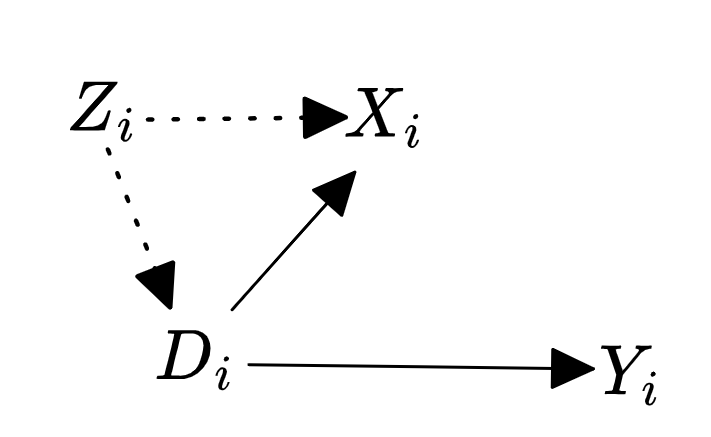
\includegraphics[width=0.3\textwidth]{figures/dag.png}

          \caption{Another figure caption.}
        \end{figure}

      \end{block}

      \begin{block}{Nam cursus consequat egestas}

        Nulla eget sem quam. Ut aliquam volutpat nisi vestibulum convallis. Nunc a
        lectus et eros facilisis hendrerit eu non urna. Interdum et malesuada fames
        ac ante \textit{ipsum primis} in faucibus. Etiam sit amet velit eget sem
        euismod tristique. Praesent enim erat, porta vel mattis sed, pharetra sed
        ipsum. Morbi commodo condimentum massa, \textit{tempus venenatis} massa
        hendrerit quis. Maecenas sed porta est. Praesent mollis interdum lectus,
        sit amet sollicitudin risus tincidunt non.

        Etiam sit amet tempus lorem, aliquet condimentum velit. Donec et nibh
        consequat, sagittis ex eget, dictum orci. Etiam quis semper ante. Ut eu
        mauris purus. Proin nec consectetur ligula. Mauris pretium molestie
        ullamcorper. Integer nisi neque, aliquet et odio non, sagittis porta justo.

        \begin{itemize}
          \item \textbf{Sed consequat} id ante vel efficitur. Praesent congue massa
                sed est scelerisque, elementum mollis augue iaculis.
                \begin{itemize}
                  \item In sed est finibus, vulputate
                        nunc gravida, pulvinar lorem. In maximus nunc dolor, sed auctor eros
                        porttitor quis.
                  \item Fusce ornare dignissim nisi. Nam sit amet risus vel lacus
                        tempor tincidunt eu a arcu.
                  \item Donec rhoncus vestibulum erat, quis aliquam leo
                        gravida egestas.
                \end{itemize}
          \item \textbf{Sed luctus, elit sit amet} dictum maximus, diam dolor
                faucibus purus, sed lobortis justo erat id turpis.
          \item \textbf{Pellentesque facilisis dolor in leo} bibendum congue.
                Maecenas congue finibus justo, vitae eleifend urna facilisis at.
        \end{itemize}

      \end{block}

    \end{column}

    \separatorcolumn

    \begin{column}{\colwidth}

      \begin{exampleblock}{A highlighted block containing some math}

        A different kind of highlighted block.

        $$
          \int_{-\infty}^{\infty} e^{-x^2}\,dx = \sqrt{\pi}
        $$

        Interdum et malesuada fames $\{1, 4, 9, \ldots\}$ ac ante ipsum primis in
        faucibus. Cras eleifend dolor eu nulla suscipit suscipit. Sed lobortis non
        felis id vulputate.

        \heading{A heading inside a block}

        Praesent consectetur mi $x^2 + y^2$ metus, nec vestibulum justo viverra
        nec. Proin eget nulla pretium, egestas magna aliquam, mollis neque. Vivamus
        dictum $\mathbf{u}^\intercal\mathbf{v}$ sagittis odio, vel porta erat
        congue sed. Maecenas ut dolor quis arcu auctor porttitor.

        \heading{Another heading inside a block}

        Sed augue erat, scelerisque a purus ultricies, placerat porttitor neque.
        Donec $P(y \mid x)$ fermentum consectetur $\nabla_x P(y \mid x)$ sapien
        sagittis egestas. Duis eget leo euismod nunc viverra imperdiet nec id
        justo.

      \end{exampleblock}

      \begin{block}{Nullam vel erat at velit convallis laoreet}

        Class aptent taciti sociosqu ad litora torquent per conubia nostra, per
        inceptos himenaeos. Phasellus libero enim, gravida sed erat sit amet,
        scelerisque congue diam. Fusce dapibus dui ut augue pulvinar iaculis.

        \begin{table}
          \centering
          \begin{tabular}{l r r c}
            \toprule
            \textbf{First column} & \textbf{Second column} & \textbf{Third column} & \textbf{Fourth} \\
            \midrule
            Foo                   & 13.37                  & 384,394               & $\alpha$        \\
            Bar                   & 2.17                   & 1,392                 & $\beta$         \\
            Baz                   & 3.14                   & 83,742                & $\delta$        \\
            Qux                   & 7.59                   & 974                   & $\gamma$        \\
            \bottomrule
          \end{tabular}
          \caption{A table caption.}
        \end{table}

        Donec quis posuere ligula. Nunc feugiat elit a mi malesuada consequat. Sed
        imperdiet augue ac nibh aliquet tristique. Aenean eu tortor vulputate,
        eleifend lorem in, dictum urna. Proin auctor ante in augue tincidunt
        tempor. Proin pellentesque vulputate odio, ac gravida nulla posuere
        efficitur. Aenean at velit vel dolor blandit molestie. Mauris laoreet
        commodo quam, non luctus nibh ullamcorper in. Class aptent taciti sociosqu
        ad litora torquent per conubia nostra, per inceptos himenaeos.



      \end{block}

      \begin{block}{References}

        \nocite{*}
        \footnotesize{\bibliographystyle{plain}\bibliography{poster}}

      \end{block}

    \end{column}

    \separatorcolumn
  \end{columns}
\end{frame}

\end{document}
